

{\setbeamercolor{background canvas}{bg=tumgraylight}
	\begin{frame}[plain]
	\vfill
	\Huge\color{tumbluedark}
	\begin{columns}
		\column{.5\textwidth}
		\vspace{4em}
		
		\hfill \textbf{Early} Time Series \\\hfill Classification
		\column{.5\textwidth}
		
\includegraphics[width=4cm]{images/TUM-blue}
		
		\vspace{1em}
		
\includegraphics[width=7cm]{images/Irisa}
	\end{columns}
	%		
\includegraphics[width=5cm]{images/TUM-white}
	%		
\includegraphics[width=7cm]{images/Irisa}
	
	\vfill
\end{frame}
}


\begin{frame}
	\frametitle{Winter Research Stay at IRISA Obelix Lab in France}
	
	\begin{columns}
		\column{.5\textwidth}
		
		Research Stay Winter 2019
		\begin{itemize}[itemsep=1em]
			\item Prof. \textbf{Sebastien Lefèvre} and Prof. \textbf{Romain Tavenard}
			\item Obelix: \textbf{Environment observation} with \textbf{complex imagery}
			\item Vannes and Rennes, Britanny, France
		\end{itemize}
		
		\vspace{1em}
		\url{http://www-obelix.irisa.fr/}
		
		\column{.5\textwidth}
		
		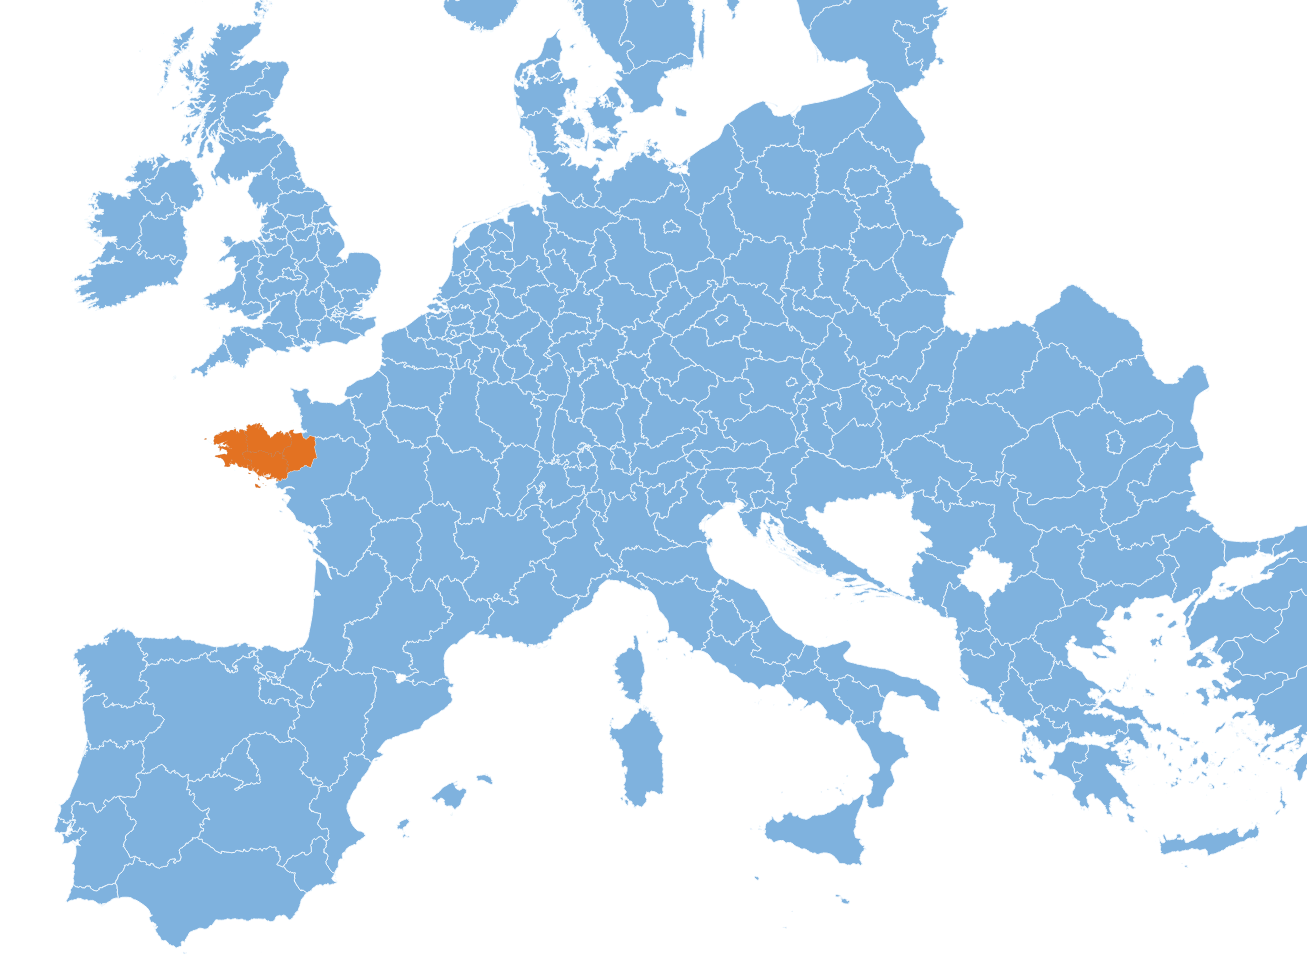
\includegraphics[width=5cm]{images/map/europe}
		
	\end{columns}
	
\end{frame}


\tikzstyle{rnn}=[draw,circle]
%\tikzstyle{annot}=[rounded corners, fill=colorblue!20]
\colorlet{colortrain}{colorblue}
\colorlet{colorinfer}{colororange}
\tikzstyle{infer}=[-stealth, shorten >=.0em, shorten <=.0em, colorinfer]
\tikzstyle{loss}=[fill=colorblue!10, rounded corners, font=\small]
\tikzstyle{grad}=[colortrain]

\newcommand{\classimagepair}[1]{
	\def\sample{#1}
	\begin{tikzpicture}[node distance=.2em]
	\node[label=above:{inputs $\V{x}_t$}](a){\includegraphics[width=.5\textwidth]{images/classification_without_earliness/TwoPatterns30EpochsNoEarliness/sample_\sample_x.png}};
	\node[label=above:{softmaxed class scores $\yhat_t$}, right=of a](b){\includegraphics[width=.5\textwidth]{images/classification_without_earliness/TwoPatterns30EpochsNoEarliness/sample_\sample_p(y).png}};
	
	\visible<2->{
		%\draw (-2,-2) to[grid with coordinates] (8,4);
		\node[annotation, yshift=3em](wiggle1) at ($ (a)!0.3!(b) $) {event \#1};
		\draw[annot] (wiggle1) -- (-1.5,0);
		\draw[annot] (wiggle1) -- (5.5,-1);
	}
	\visible<3->{
		\node[annotation, yshift=-5em](wiggle2) at ($ (a)!0.3!(b) $) {event \#2};
		\draw[annot] (wiggle2) -- (1,0);
		\draw[annot] (wiggle2) -- (7.5,0);
	}
	
	\visible<4->{
		\draw[very thick] (8.5,-2) -- (8.5,2); 
		\node[annotation, yshift=-5em, anchor=east](stop) at (10,-1) {...we could stop here};
%		\draw[shorten >=1em] (stop)++(2,0.5) -- (8,0);
	}
	\end{tikzpicture}
}

\begin{frame}<presentation:1-4>{Class Predictions}
\classimagepair{0}
\end{frame}

\begin{frame}
	\frametitle{Stopping times per crop Class}
	
	%\tikzsetnextfilename{classboxplots}

\tikzstyle{druschdatum} = [thin, star,star points=3, star point ratio=0.5, inner sep=.15em, draw=tumwhite, fill=tumblue]

\newcommand{\druschdatum}{
	\begin{tikzpicture}[scale=2, baseline=-.25em, inner sep=0]
	\node[druschdatum, inner sep=.25em]{};
	\end{tikzpicture}
}


\begin{tikzpicture}

\tikzstyle{boxstyle}=[
	mark options={
	draw=tumblue,
	scale=0.5},
	mark=*,
	solid,
	draw=black]

\begin{axis}[
ytick={1,2,3,4,5,6,7},
yticklabels={
	meadows,
	winter barley,
	corn,
	winter wheat,
	summer barley,
	clover,
	winter triticale},
xmajorgrids,
height=6cm,
xmin = 0,
xmax = 1,
ymin = 1,
ymax = 8,
width=\linewidth,
y axis line style={draw=none},
xtick={0,0.1666666667,0.4166666667,0.6666666667,0.9166666667},
xticklabels={January,March,June,September,December},
xlabel={stopping date $\tstop$}
]


%% august <- recommended end of period
% 0.6666666667
\draw [fill=tumbluelight, opacity=.4, draw=none] (axis cs:0.1666666667,0) rectangle (axis cs:0.5833333333,8);
\draw[draw=tumgraydark] (axis cs:0.5833333333,0) -- (axis cs:0.5833333333,8);

\node[font=\tiny\sffamily] at (axis cs:0.37,8.2){vegetative season};

%\node[font=\tiny\sffamily] at (axis cs:0.8,8.2){b};


\addplot+[boxplot, fill=meadowcolor, boxstyle] table[x = meadows, col sep=comma]{images/logs/data/early_reward_p2/classes/meadows.csv};
%
%\addplot+[fill=meadowcolor, draw=black,
%boxplot prepared={
%median=0.4857142857142857,
%upper quartile=0.4,
%lower quartile=0.5857142857142857,
%upper whisker=0.8642857142857143,
%lower whisker=0.12142857142857144,
%} ] coordinates {};

\addplot+[boxplot, fill=wbarleycolor, boxstyle] table[x=winter barley, col sep=comma]{images/logs/data/early_reward_p2/classes/winter_barley.csv};


%
%\addplot+[fill=wbarleycolor, draw=black,
%boxplot prepared={
%median=0.42857142857142855,
%upper quartile=0.37142857142857144,
%lower quartile=0.5857142857142857,
%upper whisker=0.9071428571428573,
%lower whisker=0.04999999999999999,
%} ] coordinates {};


\addplot+[boxplot, fill=corncolor, boxstyle] table[x =corn, col sep=comma]{images/logs/data/early_reward_p2/classes/corn.csv};
%
%\addplot+[fill=corncolor, draw=black,
%boxplot prepared={
%median=0.45714285714285713,
%upper quartile=0.42857142857142855,
%lower quartile=0.5142857142857142,
%upper whisker=0.6428571428571428,
%lower whisker=0.30000000000000004,
%} ] coordinates {};

\addplot+[boxplot, fill=wheatcolor, boxstyle] table[x =winter wheat, col sep=comma]{images/logs/data/early_reward_p2/classes/winter_wheat.csv};


%
%\addplot+[fill=wheatcolor, draw=black,
%boxplot prepared={
%median=0.5285714285714286,
%upper quartile=0.45714285714285713,
%lower quartile=0.5857142857142857,
%upper whisker=0.7785714285714287,
%lower whisker=0.26428571428571423,
%} ] coordinates {};

\addplot+[boxplot, fill=sbarleycolor, boxstyle] table[x =summer barley, col sep=comma]{images/logs/data/early_reward_p2/classes/summer_barley.csv};

%\addplot+[fill=sbarleycolor, draw=black,
%boxplot prepared={
%median=0.37142857142857144,
%upper quartile=0.2857142857142857,
%lower quartile=0.5428571428571428,
%upper whisker=0.9285714285714285,
%lower whisker=-0.09999999999999998,
%} ] coordinates {};

\addplot+[boxplot, fill=clovercolor, boxstyle] table[x=clover, col sep=comma]{images/logs/data/early_reward_p2/classes/clover.csv};

%\addplot+[fill=clovercolor, draw=black,solid,
%boxplot prepared={
%median=0.5,
%upper quartile=0.42857142857142855,
%lower quartile=0.6142857142857143,
%upper whisker=0.892857142857143,
%lower whisker=0.14999999999999986,
%} ] coordinates {};

\addplot+[boxplot, fill=triticalecolor, boxstyle] table[x=winter triticale, col sep=comma]{images/logs/data/early_reward_p2/classes/winter_triticale.csv};

\def\triticale{0.5722222222}
\def\sbarley{0.5833333333}
\def\wbarley{0.5388888889}
\def\wheat{0.5694444444}


% triticale drusch datum 26.07.
%\draw (axis cs:0.524537037,6.5) -- (axis cs:0.524537037,7.5);
\node[druschdatum] at (axis cs:\triticale,7){};

%  summer barley drusch datum 1.8.
%\draw (axis cs:\sbarley,4.5) -- (axis cs:\sbarley,5.5);
\node[druschdatum] at (axis cs:\sbarley,5){};


% winter wheat drusch datum 26.07.
%\draw (axis cs:\wheat,3.5) -- (axis cs:\wheat,4.5);
\node[druschdatum] at (axis cs:\wheat,4){};


% winter barley datum 15.07.
%\draw (axis cs:\wbarley,1.5) -- (axis cs:\wbarley,2.5);
\node[druschdatum] at (axis cs:\wbarley,2){};


%\addplot+[fill=triticalecolor, draw=black,solid,
%boxplot prepared={
%median=0.5571428571428572,
%upper quartile=0.5142857142857142,
%lower quartile=0.6142857142857143,
%upper whisker=0.7642857142857145,
%lower whisker=0.3642857142857141,
%} ] coordinates {};

\end{axis}
\end{tikzpicture} 
	
\end{frame}


\begin{frame}
\frametitle{ArXiv Paper: End-to-end Learning for Early Classification of Time Series}

\begin{columns}
	
	
	\column{.5\textwidth}
	
	Rußwurm, M., Lefèvre, S., Courty, N., Emonet, R., Körner, M., \& Tavenard, R. (2019).\textbf{ End-to-end Learning for Early Classification of Time Series}. arXiv preprint arXiv:1901.10681.
	
	\vspace{1em}
	https://github.com/rtavenar/early\_rnn
	
	\column{.5\textwidth}
	
	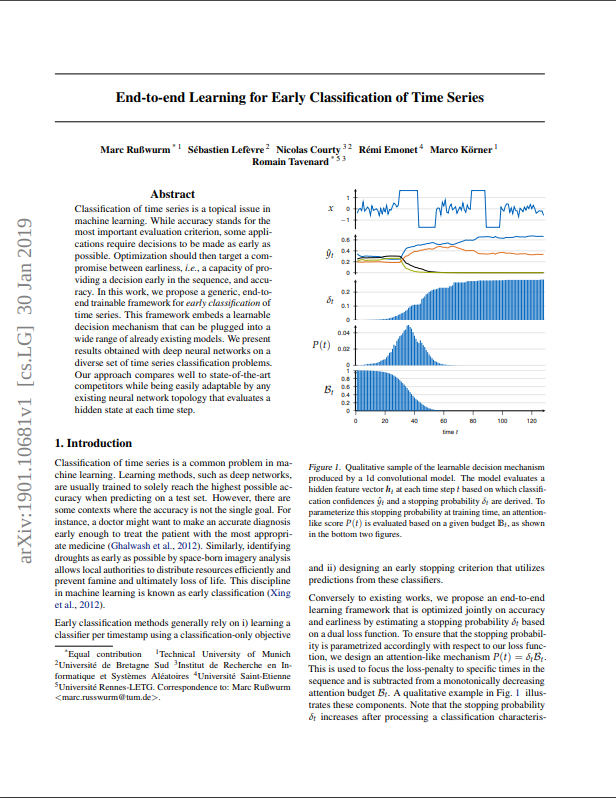
\includegraphics[width=4cm]{images/elects_arxiv}
	
\end{columns}

\end{frame}



\begin{frame}
	\frametitle{Impact of Early Classification on Vegetation Data}
	
	\Large
	
	\begin{itemize}[itemsep=1em]
		\item<1-> \bluebf{supervised end-to-end} learning scenario
		\item<2-> we get a stopping time \bluebf{for free} solely from classifying labels
		\item<3-> relate to \bluebf{characteristic features}, i.e., \bluebf{crop phenology}
		\item<4-> next: assess seasonal shifts in \bluebf{vegetation phenology} due to \bluebf{environmental conditions}
	\end{itemize}
	
\end{frame}

